% Data flow diagram
% Author: David Fokkema
\documentclass{article}
\usepackage{tikz}
\usetikzlibrary{shapes,arrows}
\usepackage{pdflscape}
\usepackage[papersize={5.5cm, 7.4cm}, text={5.5cm, 7.4cm}]{geometry}
\usetikzlibrary{decorations.text}
\usepackage{xcolor}
% \selectcolormodel{gray}

\begin{document}
\thispagestyle{empty}
%\begin{landscape}
\begin{center}
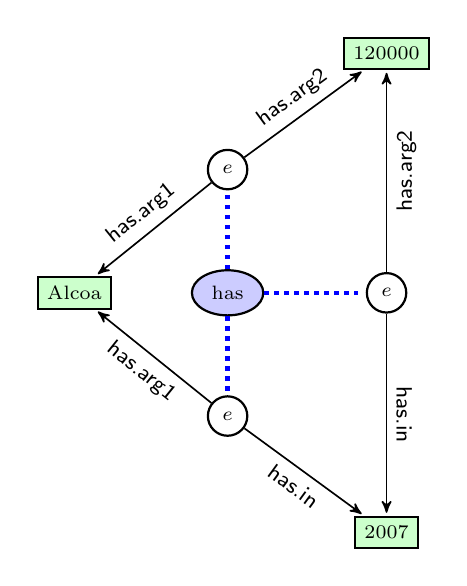
\begin{tikzpicture}[
  font=\sffamily,
  every matrix/.style={ampersand replacement=\&,column sep=1cm,row sep=1cm,font=\scriptsize},
  entity/.style={draw,thick,rectangle,fill=green!20},
  word/.style={draw,thick,ellipse,fill=blue!20},
  mediator/.style={draw,thick,circle},
  entityType/.style={draw,thick,rounded corners,fill=yellow!20,inner sep=.3cm},
  mathType/.style={draw,thick,diamond,fill=red!20},
  mediatorToEntity/.style={->,>=stealth',shorten
>=1pt,semithick,black,sloped,above,font=\sffamily\footnotesize},
  typeToEntity/.style={->,>=stealth',shorten
>=1pt,semithick,black,sloped,above,font=\sffamily\footnotesize},
  wordToEntity/.style={-,>=stealth',shorten >=1pt,ultra
thick,dotted,blue,sloped,above,font=\sffamily\footnotesize},
  entityToMath/.style={->,>=stealth',shorten >=1pt,ultra
thick,dashed,violet,sloped,above,font=\sffamily\footnotesize},
  every node/.style={align=center}]

  % Alcoa has 120,000 employees in 2007.
  
  % Position the nodes using a matrix layout
  \matrix{ 
    \&  \& \node[entity] (e120000) {120000}; \\
     \& \node[mediator] (m1) {$e$}; \&  \\
    \node[entity] (eAlcoa) {Alcoa}; \& \node[word] (wHas) {has}; \&
\node[mediator] (m2)
{$e$}; \\
     \& \node[mediator] (m3) {$e$}; \&  \\
     \&  \& \node[entity] (e2007) {2007}; \\
  };
 
  % words to entities
  % \draw [wordToEntity] (wAlcoa) edge node {}  (eAlcoa);
  %\draw [wordToEntity] (w120000) edge node {}  (e120000);
  %\draw [wordToEntity] (w2007) edge node {}  (e2007);
  
  % event word to mediators
  \draw [wordToEntity] (wHas) edge node {}  (m1);
  \draw [wordToEntity] (wHas) edge node {}  (m2);
  \draw [wordToEntity] (wHas) edge node {}  (m3);
  
  % mediator to entities
  \draw [mediatorToEntity] (m1) edge node {has.arg1}  (eAlcoa);
  \draw [mediatorToEntity] (m1) edge node {has.arg2}  (e120000);
  
  \draw [mediatorToEntity] (m2) edge node {has.in}  (e2007);
  \draw [mediatorToEntity] (m2) edge node[below] {has.arg2}  (e120000);
  
  \draw [mediatorToEntity][below] (m3) edge node {has.arg1}  (eAlcoa);
  \draw [mediatorToEntity][below] (m3) edge node {has.in}  (e2007);
  
  
  
\end{tikzpicture} 
\scriptsize $\mbox{has.arg1}(e, \mathrm{Alcoa}) \wedge \mbox{has.arg2}(e,
\mathrm{120000})$ \\ $\wedge\; \mbox{has.in}(e, \mathrm{2007})$
\end{center}

\end{document}